
\section{Translation and Ribosomal Synthesis as a Growth-Rate Limiting Step}
Thus far, the general back-of-the-envelope estimates have been reasonably
successful in predicting the scale of absolute protein copy number as well as
their observed dependence on the cellular growth rate. A recurring theme across
these varied biological processes is the ability of cells to  parallelize tasks
through the expression of additional proteins.  Even when that is not possible,
like in chromosomal replication which  requires a minimum of $\approx$ 40
minutes, \textit{E. coli} and many other bacteria surpass this limit by
initiating additional rounds of replication per doubling as we have noted. However, the synthesis
of ribosomal proteins presents a special case where parallelization is not
possible and must be doubled in quantity on average with every cell division
(\FIG{ribosome_limit}(A)).

To gain some intuition into how translation and ribosomal synthesis may limit
bacterial growth, we again consider the total number of peptide bonds that must
be synthesized, which we denote as $N_\text{pep}$. With cells growing exponentially in time
\citep{godin2010}, the rate of cellular growth will be related to the rate of protein synthesis by
\begin{equation}
    N_\text{pep} \lambda = r_t R f_a,
    \label{eq:mass_balance}
\end{equation}
where $\lambda$ is the cell growth rate in s$^{-1}$, $r_t$ is the maximum
elongation rate in AA$\cdot$s$^{-1}$, and $R$ is the average ribosome copy
number per cell. The addition factor $f_a$ refers to the fraction of actively
translating ribosomes, and allows us to account for the possibility of
nonfunctional, immature ribosomes or active sequestration of ribosomes, mediated
by the secondary-messenger molecule alarmones, guanosine pentaphosphate
[(p)ppGpp] at slow growth \citep{dennis2004, dai2016}. Knowing the number of
peptide bonds formed per cell permits us to compute the translation-limited growth
rate as
\begin{equation}
\lambda_\text{translation-limited} = \frac{r_t R f_a}{N_\text{pep}}.
\label{eq:lambda_limit}
\end{equation}

Alternatively, since $N_\text{pep}$ is related to the total protein mass through
the molecular weight of each protein, we can also consider the growth rate in
terms of the fraction of the total proteome mass dedicated to ribosomal
proteins. By making the approximation that an average amino acid has a molecular
weight of 110 Da (BNID: 104877), the total protein mass $m_{\textrm{protein}}$
is related to $N_{AA}$ by $(m_{\textrm{protein}}/\text{110 Da}) \times N_A$,
where $N_A$ is Avogadro's number. Similarly, $R$ is related to the ribosomal
protein mass by $R \approx (m_R/\text{800 Da}) \times N_A$, where 800 Da
reflects the summed molecular weight of all ribosomal subunits.  This allows us
to approximate  $R / N_\text{pep} \approx \Phi_R / L_R$,  where $\Phi_R$ is the
ribosomal mass fraction $m_{\textrm{protein}}/m_R$, and $L_R$ the ratio of 800
kDa / 110 Da per amino acid or, alternatively, the total length in amino acids
that make up a ribosome. The translation-limited growth rate can then be written
in the form
\begin{equation}
\lambda_{\textrm{translation-limited}} \approx \frac{r_t}{L_R}  \Phi_R f_a.
\label{eq:translation_limit_growth_rate}
\end{equation}
This is plotted as a function of ribosomal fraction $\Phi_R$ in
\FIG{ribosome_limit}(B), where we take $L_R$ = 7459 AA, corresponding to the
length in amino acids for all ribosomal subunits of the 50S and 30S complex
(BNID: 101175), and $f_a$ = 1. In \FIG{ribosome_limit}(C) we use the
recent measurements of $f_a$ from \cite{dai2016} to estimate the active fraction of
ribosomal protein across the proteomic data sets and number of other recent
measurements. We see that cells are consistently skirting the limit in growth
rate set by \EQ{translation_limit_growth_rate} as nutrient conditions vary.

The growth rate defined by \EQ{translation_limit_growth_rate} reflects
mass-balance under steady-state growth and has long provided a rationalization
of the apparent linear increase in \textit{E. coli}'s ribosomal content as a
function of growth rate \citep{goldberger1979, scott2010}. The maximum rate,
when $\Phi_R$ = 1, could only be achieved if a cell contained only ribosomes.
This corresponds to the synthesis time of all ribosomal subunits, $L_R/ r_t
\approx$ 7 minutes \citep{dill2011} and interestingly, is independent of the
absolute number of ribosomes.  This is because, in order to double the cell's
ribosomal mass, each ribosome must produce a second ribosome; a process which
cannot be parallelized. Unless elongation rate increased, or cells could trim
their total ribosomal protein mass, this dependency limits both the maximum
growth rate (when $\Phi_R$ = 1), and also the achiveable growth rate under more
realistic values of $\Phi_R$.

\begin{figure}
  \begin{fullwidth}
        \centering{
            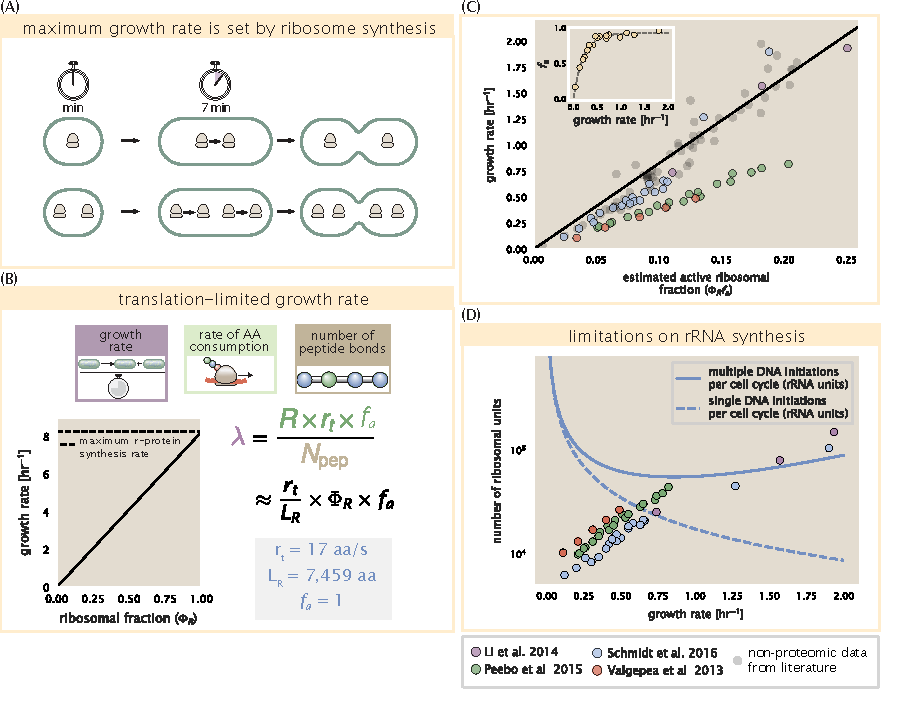
\includegraphics{main_figs/fig7_ribosome_as_limit.pdf}
            \caption{\textbf{Translation-limited growth rate.}  (A) An inherent
            maximum growth rate is set by the time to synthesize all ribosomal
            subunits. This growth rate is given by $r_t/ L_R$, where $r_t$ is
            the elongation rate and $L_R$ is the total number of amino acids
            that make up the entire ribosomal complex. This rate is independent
            of the number of ribosomes; instead limited serial requirement for
            each ribosome to double itself. (B)
            Translation-limited growth as a function of the ribosomal fraction. The
            solid line is calculated for an elongation rate of 17 aa per second.
            The dashed line corresponds to the maximum rate of ribosomal protein
            (R-protein) synthesis considered in part (A).
            (C) Actively translating ribosomal fraction versus growth rate.
            The actively translating ribosomal fraction is calculated using the
            estimated values of $f_a$ from  \cite{dai2016} (shown in inset; see
            Appendix \nameref{sec:SI_f_a} for additional detail).
            (D) Maximum number of
            rRNA units that can be synthesized as as a function of growth rate.
            Solid curve corresponds to the rRNA copy number is calculated by
            multipyling the number of rRNA operons by the estimated number of
            $\langle\text{\# ori}\rangle$ at each growth rate. The quantity
            $\langle\text{\# ori}\rangle$ was calculated using Equation 4 and
            the measurements from \cite{si2017} that are plotted in
            \FIG{translation_ecoli_partA}(A). The dashed line shows the maximal
            number of functional rRNA units produced from a single chromosomal
            initiation per cell cycle. }
        \label{fig:ribosome_limit}
        }
  \end{fullwidth}
\end{figure}

This strain of \textit{E. coli} rarely exhibits growth rates above 2 hr$^{-1}$
\citep{bremer2008,roller2016} and in \FIG{ribosome_limit}(C) we consider
ribosomal generation from the perspective of rRNA synthesis. Here we use our
rule-of-thumb of 1 functional rRNA unit per second per operon and estimate the
maximum number of ribosomes that could  be made as a function of growth rate
(blue curve).  Although we expect this estimate to drastically overestimate rRNA
abundance at slower growth rates ($\lambda < 0.5\, \text{hr}^{-1}$), it provides
a useful reference alongside the proteomic measurements. For growth rates above
about 1 hr$^{-1}$, we find that cells will need to transcribe rRNA near their
maximal rate. As a counter example, if \textit{E. coli} did not initiate
multiple rounds of replication, they would be unable to make enough rRNA for the
observed number of ribosomes (dashed blue curve in \FIG{ribosome_limit}(C)). The
convergence between the maximum rRNA production and measured ribosome copy
number suggests rRNA synthesis may begin to present a bottleneck at the fastest
growth rates due to the limited copies of rRNA genes.
